\chapter{Технологический раздел}
В этом разделе будет обоснован выбор языка программирования и среды разработки, рассмотрена диаграмма основных классов и разобран интерфейс, предлагаемый пользователю.

\section{Требования к программе} 
Программа должна предоставлять следующие возможности:
\begin{itemize}
	\item визуальное отображение сцены;
	\item запуск и остановка ударов молнии;
	\item возможность включения и выключения света во всех окнах дома;
	\item поворот исходной сцены.
\end{itemize}

\section{Выбор языка программирования и среды разработки}
Существует множество языков, а также сред программирования, многие из которых обладают достаточно высокой эффективностью, удобством и простотой в использовании. Для разработки данной программы был выбран язык C\# \cite{csharplang}. Данный выбор обусловлен следующими факторами.

\begin{enumerate}
	\item Этот язык предоставляет программисту широкие возможности реализации самых разнообразных алгоритмов. Он обладает высокой эффективностью и большим набором стандартных классов и процедур.
	\item C\# является полностью объектно-ориентированным. Он позволяет использовать множественное наследование, абстрактные и параметризованные классы.
	\item Язык является строго типизированным, что позволяет защититься от неконтролируемых  ошибок.
	\item В данном языке имеется большое количество библиотек и шаблонов, позволяющих не тратить время на изобретение готовых конструкций.
\end{enumerate}

В качестве среды разработки была выбрана Visual Studio 2019. Некоторые факторы по которым была выбрана данная среда.
\begin{enumerate}
	\item Включает весь основной функционал: параллельная сборка, отладчик, поддержка точек останова, сборки и т.д.
	\item Разработчики имеют возможность расширить любой функционал, включая компиляцию, отладку.
	\item Работает с интерфейсом Windows Forms, который очень удобен в использовании, а также позволяет без проблем создавать приложения.
\end{enumerate}

\section{Структура программы}
Так как при написании программы используется язык C\#, а это объектно-ориентированный язык, то особое внимание уделено структуре классов.

Условно классы в программе можно разделить на несколько групп по выполняемым функциям.
  
\begin{itemize}
	\item Математические абстракции
	\begin{itemize}
		\item Trace - структура, в которую входит точка пересечения луча с объектом расстояние от камеры до точки пересечения
		\item Ray - трехмерный луч, задающийся точкой начала луча, направляющим вектором
		\item Comparator - помогает сравнивать сегменты молнии
	\end{itemize}
	\item Вспомогательные классы свойств трехмерных объектов
	\begin{itemize}
		\item Texture - абстрактный класс с основными свойствами.
		\item SimpleTexture и VectorTexture - обеспечивают загрузку из файла текстуры, ее интерпретацию на простую поверхность
	\end{itemize}
	\item Трехмерные объекты
	\begin{itemize}
		\item House – реализует работу с домом, генерацию, трехмерные преобразования
		\item Lightning – реализует работу с молнией, генерацию, трёхмерные преобразования.
	\end{itemize}
	\item Источники света
	\begin{itemize}
		\item Shadow - класс, позволяющий работать с тенями. Одним из ключевых механизмов базового алгоритма обратной трассировки лучей является метод теневых лучей, позволяющие реализовать тени от загораживающих источники света объектов.
	\end{itemize}
	\item Сцена
	\begin{itemize}
		\item Scene - характеризует набор объектов и их свойств. Следует обратить внимание на то, что сцена использует динамические объекты, что позволяет уже после загрузки и построения сцены изменить ее состав (удалять/добавлять/изменять компоненты).
	\end{itemize}
	\item Алгоритмы визуализации
	\begin{itemize}
		\item Highlight - отрисовка вспышки
		\item Lightning - отрисовка молнии
		\item House - отрисовка дома
		\item Shadow - отрисовка тени
		\item Texture - отрисовка текстуры
		\item Window - отрисовка окна
	\end{itemize}
	\item Интерфейс пользователя
	\begin{itemize}
		\item Взаимодействие с интерфейсом происходит через диалоговые окна, которые в свою очередь взаимодействуют с классом Scene
	\end{itemize}	
\end{itemize}

На рисунке \ref{img:shema} представлена структура и состав классов (!!!повернуть).

\img{240mm}{shema}{Структура и состав классов}
\clearpage

\section{Интерфейс}
На рисунке \ref{img:inter} представлен интерфейс программы.

\img{100mm}{inter}{Интерфейс программы}

Функции представленных кнопок следующие:
\begin{itemize}
	\item кнопка ''Запустить/Остановить'' -- запускает или выключает (останавливает) автоматическую генерацию молнии, непрерывно генерируются различные изображения;
	\item кнопка ''Визуализация'' -- создает одно изображение с указанной частотой включения и выключения света в окнах;
	\item кнопка ''Включить свет'' -- включает свет во всех окнах;
	\item кнопка ''Выключить свет'' -- выключает свет во всех окнах;
	\item кнопка ''Изменить количество этажей'' -- изменяет высоту дома (количество этажей), значение берется из поля слева, при этом генерируется новая сцена.
	\item поле ''Частота смены освещения'' -- указывает с каким периодом (в тактах) будет изменяться количество окон, в которых горит свет. По умолчанию пользователь может либо включить во всех окнах свет, либо выключить;
	\item поле ''?'' -- справка по управлению программы с помощью клавиатуры.
\end{itemize}

Корректность ввода данных проверяется автоматически за счет средств, предоставляемых интерфейсом Windows Forms. 

Также пользователь может взаимодействовать с программой при помощи стрелок вправо/влево или кнопок ''A'' и ''D'' на клавиатуре. Таким образом будет производиться поворот сцены.


\section{Результаты работы программного обеспечения}

На рисунке \ref{img:t1} приведен результат генерации сцены, на которой показана молния-лидер.

\begin{figure}[H]
	\begin{center}
		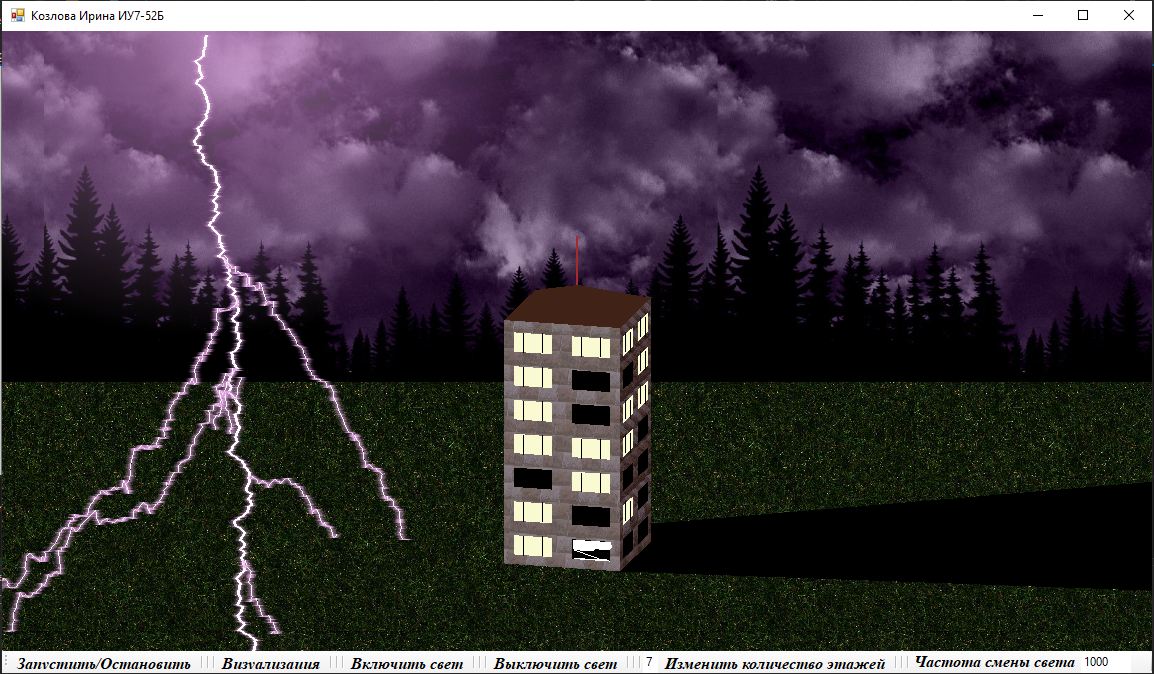
\includegraphics[scale=0.38]{img/prog_res/t1.png}
	\end{center}
	\captionsetup{justification=centering}
	\caption{Изображение с молнией-лидером}
	\label{img:t1}
\end{figure}

На рисунке \ref{img:t2} приведен результат генерации сцены, на котором видно отражение молнии от стекол окон дома.

\begin{figure}[H]
	\begin{center}
		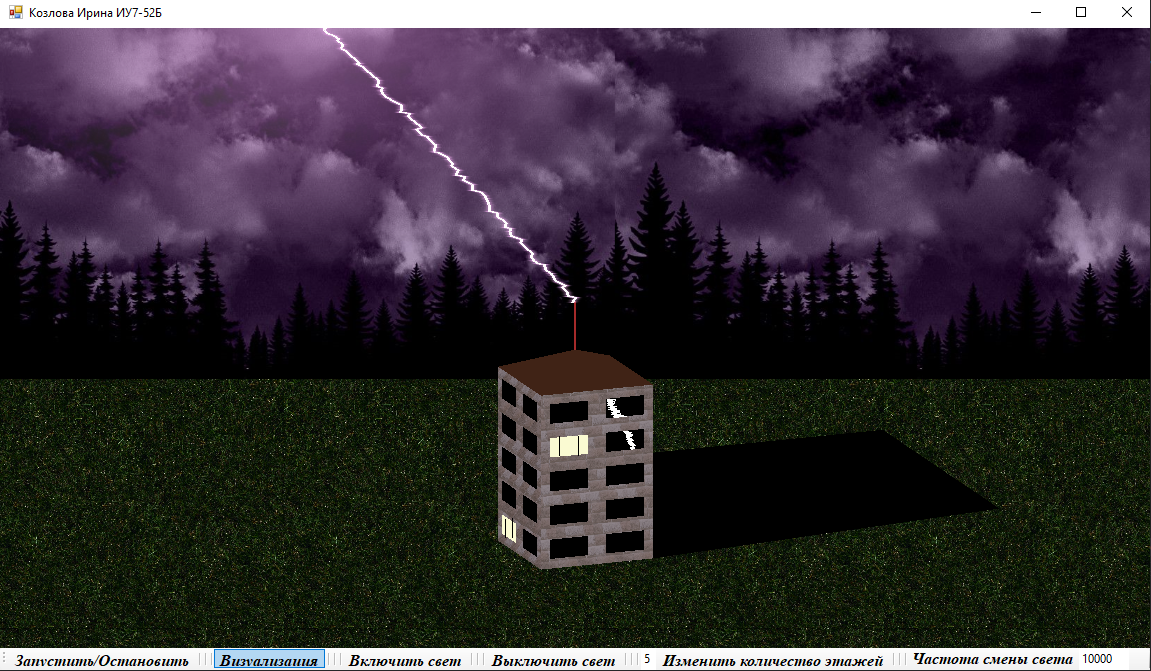
\includegraphics[scale=0.38]{img/prog_res/t2.png}
	\end{center}
	\captionsetup{justification=centering}
	\caption{Изображение с отражением молнии от стекл окон дома}
	\label{img:t2}
\end{figure}

На рисунке \ref{img:t3} приведен результат генерации сцены, на которой показана молния, бьющая в громоотвод.

\begin{figure}[H]
	\begin{center}
		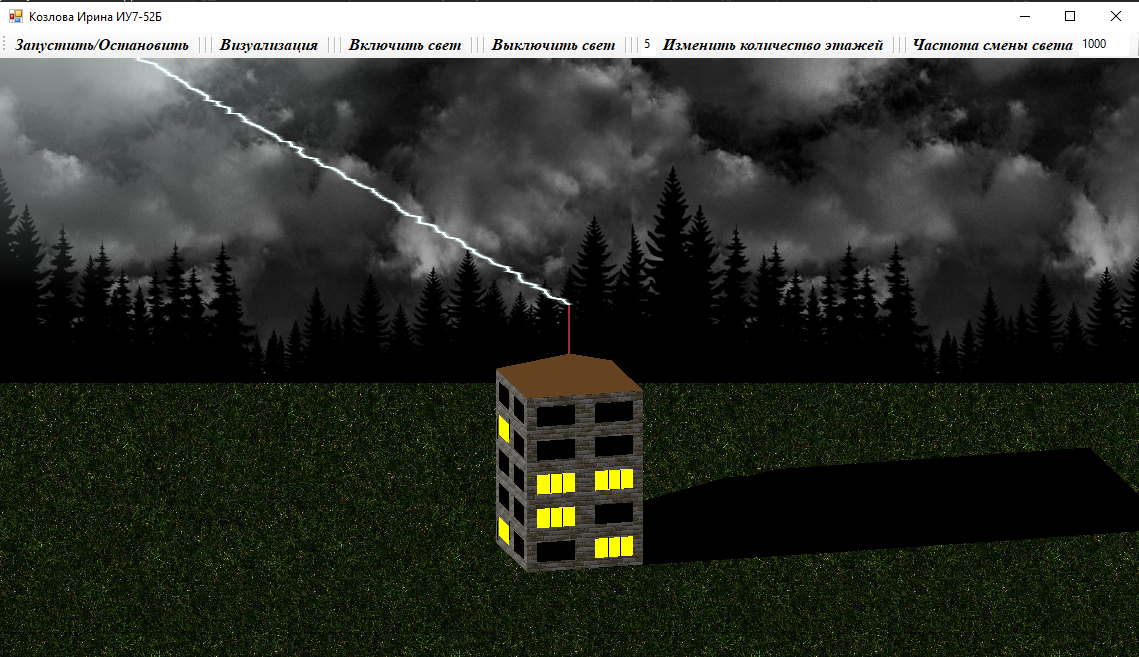
\includegraphics[scale=0.38]{img/prog_res/t3.png}
	\end{center}
	\captionsetup{justification=centering}
	\caption{Изображение с молнией, бьющей в громоотвод}
	\label{img:t3}
\end{figure}

На рисунке \ref{img:t4} приведен результат генерации сцены, на которой показана молния с большим количеством побочных ветвей.

\begin{figure}[H]
	\begin{center}
		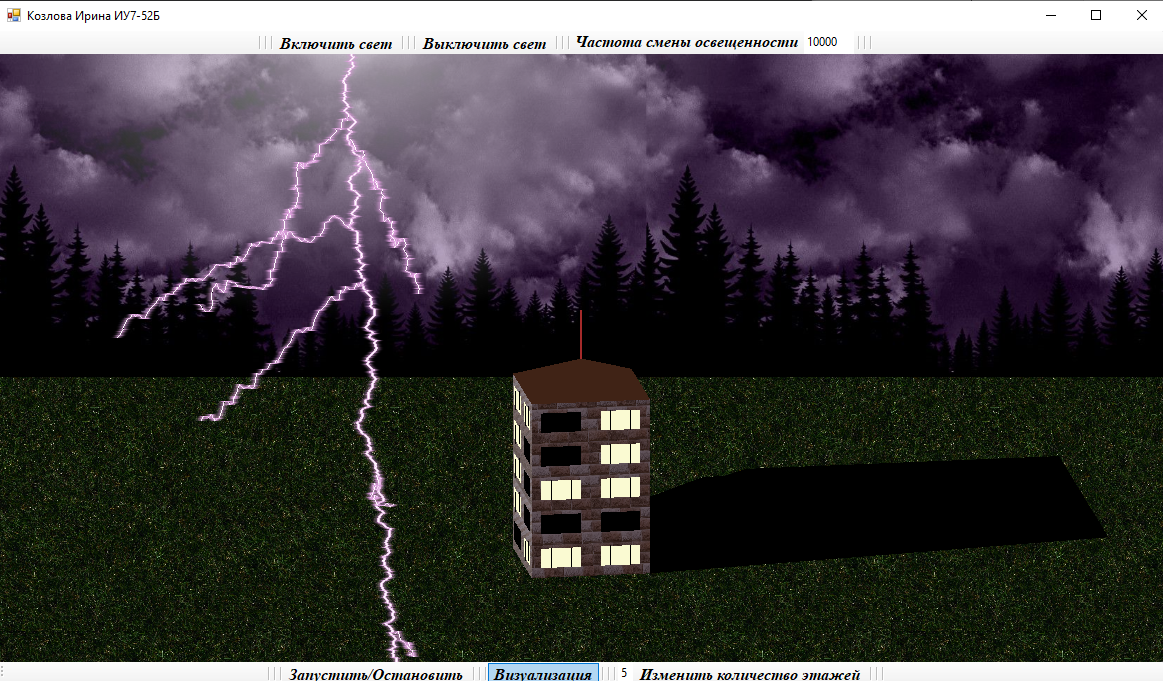
\includegraphics[scale=0.38]{img/prog_res/t4.png}
	\end{center}
	\captionsetup{justification=centering}
	\caption{Изображение с молнией, у которой большое количество ветвей}
	\label{img:t4}
\end{figure}


\section{Вывод}
В этом разделе был выбран язык программирования и среда разработки, рассмотрена uml-диаграмма основных классов, подробно разобран интерфейс приложения и приведены результаты работы програмы.